\subsection{Results I:  The Experiment}

\label{sec:results}

This section reports results of analyzing 945 jar libraries extracted from
Debian 6.0 Squeeze to answer the research questions formulated 
%-- in Section~\ref{sec:method}.  
at the beginning of this section.
By treating version and name information encoded
in the 945 Debian jar files as a good approximation of ground truth, we can
compare our signature-based Bertillonage technique against a baseline
technique.

Our techniques consider only the top match according to our
\emph{similarity} metric, as described in Section~\ref{sec:sim}.  Often the
top similarity score is shared by several artifacts in our corpus.  As
evidenced by the results, 2-way, 3-way, and 4-way ties for best similarity are the
norm, rather than the exception.  However, to understand what we mean by a
\emph{tie}, we must mention briefly what we consider \emph{a single
artifact}.  Our earlier exploration of the Maven2 corpus (see
Section~\ref{sec:mavenExplore}) shows surprising redundancy and duplication
of archives within the repository.  Users are likely not interested in knowing all two hundred
path locations of an identical artifact.  We filter out these duplications
and instead report only ties that either have a different SHA1 binary
fingerprint than other matches in the tie, or a different name.  

In some cases choosing a top match based on the inclusion metric rather
than similarity performs better.  To keep our experiment simple, we
consider these to be wrong matches.  We anticipate future researchers
will improve on our results by tuning the match criteria to factor in
both similarity and inclusion scores when selecting the \emph{top} match,
perhaps at a cost of larger \emph{ties}.


\subsubsection{The Baseline:  Binary Fingerprint Matches}

\begin{table}[h]
  \centering
\begin{tabular}[htbp]{l|r|lll|rrr}
  sha1-of-class/Debian-945   &              & \multicolumn{3}{c|}{\textbf{Similarity}}  & \multicolumn{3}{c}{\textbf{\# of Ties}} \\
  \textbf{Type of Match}     & Count        & Min   & Mdn    & Max   & Min  & Mdn  & Max  \\
\hline
%& & & & & & & \\
  \emph{HQ1.} Identical archive          &   2          & 1.0   & 1.0    & 1.0   & 1    & 1    &  1   \\
  \emph{HQ2.} Identical contents         & 201          & 1.0   & 1.0    & 1.0   & 1    & 1    & 35   \\
  \emph{HQ3.} Expected match             & 131          & 0.014 & 0.680  & 0.997 & 1    & 1    & 13   \\
  \emph{HQ4.} Version off by final digit &  49          & 0.033 & 0.500  & 0.977 & 1    & 1    &  4   \\
  \emph{\textbf{High Quality Matches}}   & \textbf{383} &       &        &       &      &      &      \\
& & & & & & & \\
  \emph{LQ1.} Version off by many digits &  85          & 0.001 & 0.116  & 0.964 & 1    & 1    & 25   \\
  \emph{LQ2.} Not useful                 &  22          & 0.003 & 0.025  & 0.206 & 1    & 1    & 18   \\
  \emph{\textbf{Low Quality Matches}}    & \textbf{107} &       &        &       &      &      &      \\
& & & & & & & \\
  \emph{\textbf{No Matches}}             & \textbf{455} &       &        &       &      &      &     \\
%& & & & & & & \\
\hline
  \textbf{Total Matches:} \hspace{3em} \textbf{(52\%)} & \textbf{490}   & \multicolumn{3}{c|}{\textbf{Average: 0.685}}  & \multicolumn{3}{c}{\textbf{Average: 2.4}} \\
\end{tabular}
  \caption{The baseline results:  matches are based on binary SHA1 fingerprints of the 945 Debian jars.}
  \label{tab:debianSha1OfClass}
\end{table}


\begin{table}[h]
  \centering
\begin{tabular}[htbp]{r|r|r}
\textbf{Tie \#}  & \textbf{Similarity} & \multicolumn{1}{c}{\textbf{Version}} \\
\hline
1.        & 1.0 &          plexus-component-annotations-1.0-alpha-1.jar  \\
2. - 17.  & 1.0 &                            \multicolumn{1}{c}{\emph{alpha-2 - alpha-17}}  \\
18.       & 1.0 &           plexus-component-annotations-1.0-beta-1.jar  \\
19. - 27. & 1.0 &                   \multicolumn{1}{c}{\emph{1.0-beta-2 - 1.0-beta-3.0.6}}  \\
\textbf{28.}       & \textbf{1.0} &       \textbf{plexus-component-annotations-1.0-beta-3.0.7.jar}  \\
29. - 34. & 1.0 &                                 \multicolumn{1}{c}{\emph{1.0 - 1.2.1.3}}  \\
35.       & 1.0 &              plexus-component-annotations-1.2.1.4.jar  \\
\end{tabular}
  \caption{
    We found 35 top matches with
    \mytt{plexus-component-annotations-1.0-beta- 3.0.7.jar} when using
    binary fingerprint matches.  Notice how candidate \#28 contains the
    same name as the subject archive, hence this match could be classified
    as `HQ3. Expected Match.' However, we consider all 1.0 similarity
    matches of SHA1 fingerprints as ground truth, hence this match's
    classification as `HQ2. Identical Contents.' A relatively small jar,
    \mytt{plexus-component-annotations-1.0-beta-3.0.7.jar} contains only 3
    classes.  
}
  \label{tab:sha1-of-class-35-matches}
\end{table}

Table \ref{tab:debianSha1OfClass} shows the results of our baseline
technique, a straightforward SHA1 index of jar files and class files.
Slighly over half the Debian sample, 490 jars out of 945 (52\%), contained
one or more class files that were identical to a class file in the Maven
corpus.  Each match returned an average of 2.4 candidates that tied for top
similarity.  The match with the most ties among our baseline results is
shown in Table \ref{tab:sha1-of-class-35-matches}.  The average score of
the 490 best similarity scores was 0.685.

Only 2 out of the 945 jar files proved to be identical complete archive
copies from the Maven corpus (row \emph{HQ1}).  We suspect the main reason
for such a low match percentage (less than 0.5\%) in this category may be
Debian's policy of recompiling all jar files from original sources.  Jar
files record timestamps of contained files, and Java class files tend to
have timestamps set to the moment they were compiled.  This alone will
cause Debian jar files to differ, at least in a few bytes, from their Maven
counterparts.  A further 201 out of the 945 jar files matched with
identical contents (\emph{HQ2}).  These 201 matches, while externally
different, were internally identical with respect to contained class files.
Of course the 2 identical jar files also matched according to contents.

A remaining 287 jar files had partial matches, with similarity scores less
than 1.0.  Of these, 180 matches, when evaluated against our ground truth,
scored as high quality matches (\emph{HQ3} to \emph{HQ4}), and 107 matches
scored as low quality matches (\emph{LQ1} to \emph{LQ2}).  Finally, for 455
jars, there were no matches at all using the binary fingerprint technique.


\subsubsection{The First Test: Binary-to-Binary Anchored Signature}

\begin{table}[h]
  \centering
\begin{tabular}[htbp]{l|r|lll|rrr}
  bin2bin/Debian-945         &              & \multicolumn{3}{c|}{\textbf{Similarity}}  & \multicolumn{3}{c}{\textbf{\# of Ties}} \\
  \textbf{Type of Match}     & Count        & Min   & Mdn    & Max   & Min  & Mdn  & Max  \\
  \hline
%& & & & & & & \\
  \emph{HQ1.} Exact (sha1 of jar)        &   2          & 1.0   & 1.0    & 1.0   & 1    & 1.5  &  2   \\
  \emph{HQ2.} Exact (sha1 of *.class)    & 201          & 1.0   & 1.0    & 1.0   & 1    & 3    & 86   \\
  \emph{HQ3.} Expected match             & 442          & 0.046 & 1.0    & 1.0   & 1    & 2    & 30   \\
  \emph{HQ4.} Version off by final digit &  65          & 0.038 & 0.889  & 1.0   & 1    & 1    & 23   \\
  \emph{\textbf{High Quality Matches}}   & \textbf{710} &       &        &       &      &      &      \\
& & & & & & & \\
  \emph{LQ1.} Version off by many digits &  67          & 0.014 & 0.414  & 1.0   & 1    & 1    & 14   \\
  \emph{LQ2.} Not useful                 &  16          & 0.002 & 0.027  & 0.807 & 1    & 1    &  4   \\
  \emph{\textbf{Low Quality Matches}}    & \textbf{83}  &       &        &       &      &      &      \\
& & & & & & & \\
  \emph{\textbf{No Matches}}             & \textbf{152} &       &        &       &      &      &     \\
%& & & & & & & \\
  \hline
  \textbf{Total Matches:} \hspace{3em}    \textbf{(84\%)} &  \textbf{793}   & \multicolumn{3}{c|}{\textbf{Average: 0.890}}  & \multicolumn{3}{c}{\textbf{Average: 3.5}} \\
\end{tabular}
  \caption{bin2bin Bertillonage --- our signature-based approach applied to
    945 Debian jars.} 
  \label{tab:debianBin2Bin}
\end{table}


\begin{table}[h]
  \centering
\begin{tabular}[htbp]{r|r|l|l}
\textbf{Match \#}  & \textbf{Similarity} & \textbf{Inclusion} & \multicolumn{1}{c}{\textbf{Match}} \\
\hline
1.        & 0.046 & 1.0   &         javahelp-2.0.05.jar \\
2.        & 0.041 & 0.889 &         javahelp-2.0.02.jar \\
\end{tabular}
  \caption{
    In this anchored signature example the top match for
    \mytt{jsearch-indexer-2.0.05.ds1.jar} had a low similarity score. Only
    9 of \mytt{javahelp-2.0.05.jar}'s 195 signatures matched.  We
    classified this as HQ3. ``Expected match,'' since it resided inside a
    Debian package named \mytt{javahelp2\_2.0.05.ds1-4\_all.deb}, and so
    name and version did match as expected.  Because this match also
    possessed a 1.0 inclusion score, we suspect the Debian maintainers are
    splitting a large jar (which exists in Maven) into several smaller jars
    (which do not).  }
  \label{tab:046similarity}
\end{table}

Table \ref{tab:debianBin2Bin} shows the results of our first Bertillonage
test:  binary-to-binary anchored signature matching.  In the Debian sample,
we found that 793 jars out of 945 (84\%) contained one or more class files
with an identical anchored signature as a class file in the Maven corpus.
Each match returned an average of 3.5 candidates that tied for top
similarity.  The average score of the 793 best similarity scores was
0.890.  The highest quality match with the lowest similarity score (0.046)
is shown in table \ref{tab:046similarity}.

We found that 710 matches, when evaluated against our ground truth, scored
as high quality matches (\emph{HQ1} to \emph{HQ4}), and 83 matches scored
as low quality matches (\emph{LQ1} to \emph{LQ2}).  Finally, for 152 jars,
there were no matches at all using anchored signature binary-to-binary
matches.  In general our Bertillonage approach outperformed the baseline,
with nearly twice as many high-quality matches (710 vs.\ 383), fewer
low-quality matches (83 vs.\ 107), and far fewer non-matches (152 vs.\ 455).

As expected, all binary-identical matches also scored 1.0 for
signature-similarity, as shown in the two crosstab rows (\emph{HQ1} to
\emph{HQ2}).  Any non-perfect score in these rows would signify a critical
bug in our tool, since a binary-identical class-file should also possess an
identical signature.  One interesting difference, however, is the increase
in ties in the crosstab rows.  The anchored signature approach exhibited a
higher median (3 vs.\ 1), a higher maximum (86 vs.\ 35), and the overall
average tie rate was also higer (3.5 vs.\ 2.4).  These differences highlight
the tradeoff anchored signature provides:  higher recall (e.g., 793 vs.\ 450
total matches), but in exchange the user must do more work analyzing the
results (3.5 ties to examine vs.\ 2.4 ties).



\subsubsection{The Second Test: Binary-to-Source Anchored Signature}


\begin{table}[h]
  \centering
\begin{tabular}[htbp]{l|r|lll|rrr}
  bin2src/Debian-945                     &       & \multicolumn{3}{c|}{\textbf{Similarity}}  & \multicolumn{3}{c}{\textbf{\# of Ties}} \\
  \textbf{Type of Match}                 & Count & Min   & Mdn   & Max   & Min & Mdn  & Max  \\
  \hline
%& & & & & & & \\
  \emph{HQ1.} Exact (sha1 of jar)        & \multicolumn{1}{c|}{\emph{n/a}} & & \emph{n/a} & & & \emph{n/a} &  \\
  \emph{HQ2.} Exact (sha1 of *.class)    & & & & & & & \\
  \emph{HQ3.} Expected match             & 443   & 0.001 & 1.0   & 1.0   & 1   & 2    & 77   \\
  \emph{HQ4.} Version off by final digit &  84   & 0.018 & 0.750 & 1.0   & 1   & 1    &  2   \\
  \emph{\textbf{High Quality Matches}}   & \textbf{527} &       &        &       &      &      &      \\
& & & & & & & \\
  \emph{LQ1.} Version off by many digits & 109   & 0.001 & 0.326 & 1.0   & 1   & 1    & 20   \\
  \emph{LQ2.} Not useful                 &  24   & 0.002 & 0.136 & 0.886 & 1   & 1.5  & 20   \\
  \emph{\textbf{Low Quality Matches}}    & \textbf{133} &       &        &       &      &      &      \\
& & & & & & & \\
  \emph{\textbf{No Matches}}             & \textbf{285} &       &        &       &      &      &     \\
%& & & & & & & \\
  \hline
  \textbf{Total Matches:} \hspace{3em}    \textbf{(70\%)} &  \textbf{660}  & \multicolumn{3}{c|}{\textbf{Average: 0.773}}  & \multicolumn{3}{c}{\textbf{Average: 2.9}} \\
\end{tabular}
  \caption{bin2src Bertillonage --- our signature-based approach applied to
    945 Debian jars.}
  \label{tab:debianBin2Src}
\end{table}

\begin{table}[h]
  \centering
\begin{tabular}[htbp]{r|r|l|l}
\textbf{Match \#}  & \textbf{Similarity} & \textbf{Inclusion} & \multicolumn{1}{c}{\textbf{Match}} \\
\hline
1.        & 0.001 & 1.0   &         org.apache.ant.source\_1.7.1.jar \\
\end{tabular}
  \caption{
    In this anchored signature binary-to-source example the best (and only)
    match for \mytt{ant-apache-log4j-1.7.1.jar}, a jar containing a single
    class, had an extremely low similarity score.  The source archive
    contained 791 signatures.  We classified this as HQ3. ``Expected
    match,'' since the name and version were correct.  We suspect
    \mytt{ant}'s own internal build script creates these tiny single-task
    jar files.
}
  \label{tab:001similarity}
\end{table}


Table \ref{tab:debianBin2Src} shows the results of our second Bertillonage
test:  binary-to-source anchored signature matching.  In the Debian sample,
we found that 660 jars out of 945 (70\%) contained one or more class files
with an identical anchored signature as a \emph{source} file in the Maven
corpus.  Each match returned an average of 2.9 candidates that tied for top
similarity.  The average score of the 660 best similarity scores was
0.773.  The highest quality match with the lowest similarity score (0.001)
is shown in table \ref{tab:001similarity}.

We found that 527 matches, when evaluated against our ground truth, scored
as high quality matches (\emph{HQ3} to \emph{HQ4}), and 133 matches scored
as low quality matches (\emph{LQ1} to \emph{LQ2}).  Finally, for 285 jars,
there were no matches at all using anchored signature binary-to-binary
matches.  In general our binary-to-source Bertillonage approach
outperformed the baseline, with 40\% more high-quality matches (527 vs.\
383), fewer non-matches (285 vs.\ 455), but increased low-quality matches
(133 vs.\ 107).



\begin{figure}[ht]
\begin{minipage}[b]{0.5\linewidth}
\centering
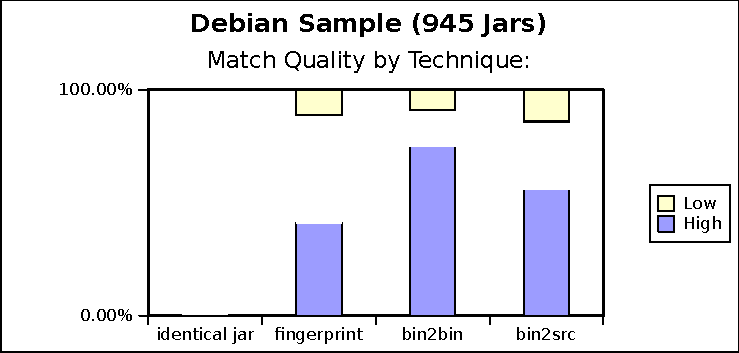
\includegraphics[width=\columnwidth]{plots/debianMatchQuality.pdf}
\end{minipage}
\hspace{0.5cm}
\begin{minipage}[b]{0.5\linewidth}
\centering
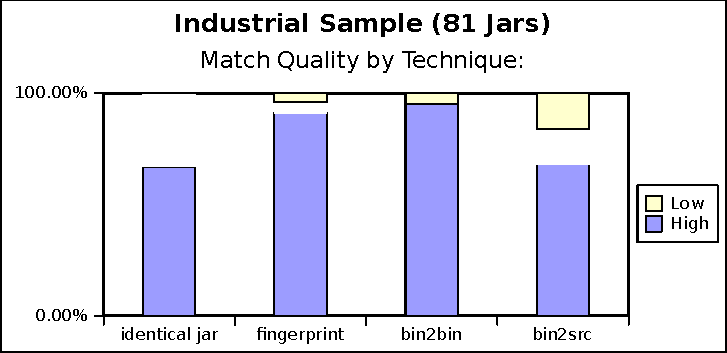
\includegraphics[width=\columnwidth]{plots/industryMatchQuality.pdf}
\end{minipage}
\vspace{-2mm}
\caption{A comparison of match quality by data set.  Left: Debian's 945
    jars.  Right: Industry's 81 jars.  The Industry set receives a boost of
    77\% binary-identical matches compared to Debian's 21\%.  Aside from
    this boost, the results appear similar.}
\label{fig:matchQuality}
\end{figure}


\subsection{Results II:  Industry Case Study, A Replication}

\begin{table}[h]
  \centering
\begin{tabular}[htbp]{l|r|lll|rrr}
  sha1-of-class/Industry-81  &              & \multicolumn{3}{c|}{\textbf{Similarity}}  & \multicolumn{3}{c}{\textbf{\# of Ties}} \\
  \textbf{Type of Match}     & Count        & Min   & Mdn    & Max   & Min  & Mdn  & Max  \\
  \hline
%& & & & & & & \\
  \emph{HQ1.} Exact (sha1 of jar)        & 54           & 1.0   & 1.0    & 1.0   & 1    & 2    & 14   \\
  \emph{HQ2.} Exact (sha1 of *.class)    &  9           & 1.0   & 1.0    & 1.0   & 1    & 1    &  5   \\
  \emph{HQ3.} Expected match             &  4           & 0.006 & 0.758  & 0.965 & 1    & 1.5  &  4   \\
  \emph{HQ4.} Version off by final digit &  7           & 0.016 & 0.500  & 0.962 & 1    & 1    & 12   \\
  \emph{\textbf{High Quality Matches}}   & \textbf{74}  &       &        &       &      &      &      \\
& & & & & & & \\
  \emph{LQ1.} Version off by many digits &  1           & 0.038 & 0.038  & 0.038 & 1    & 1    &  1   \\
  \emph{LQ2.} Not useful                 &  2           & 0.002 & 0.031  & 0.059 & 1    & 1    &  1   \\
  \emph{\textbf{Low Quality Matches}}    & \textbf{3}   &       &        &       &      &      &      \\
& & & & & & & \\
  \emph{\textbf{No Matches}}             & \textbf{4}   &       &        &       &      &      &      \\
%& & & & & & & \\
  \hline
  \textbf{Total Matches:} \hspace{3em}   \textbf{(95\%)} &  \textbf{77}   & \multicolumn{3}{c|}{\textbf{Average: 0.903}}  & \multicolumn{3}{c}{\textbf{Average: 2.8}} \\
   \multicolumn{8}{c}{} \\
   \multicolumn{8}{c}{} \\
  bin2bin/Industry-81        &              & \multicolumn{3}{c|}{\textbf{Similarity}}  & \multicolumn{3}{c}{\textbf{\# of Ties}} \\
  \textbf{Type of Match}     & Count        & Min   & Mdn    & Max   & Min  & Mdn  & Max  \\
  \hline
%& & & & & & & \\
  \emph{HQ1.} Exact (sha1 of jar)        & 54           & 1.0   & 1.0    & 1.0   & 1    & 3    & 16   \\
  \emph{HQ2.} Exact (sha1 of *.class)    &  9           & 1.0   & 1.0    & 1.0   & 1    & 1    &  9   \\
  \emph{HQ3.} Expected match             &  6           & 0.933 & 0.994  & 1.0   & 1    & 1    &  2   \\
  \emph{HQ4.} Version off by final digit &  8           & 0.133 & 0.915  & 1.0   & 1    & 1    & 12   \\
  \emph{\textbf{High Quality Matches}}   & \textbf{77}  &       &        &       &      &      &      \\
& & & & & & & \\
  \emph{LQ1.} Version off by many digits &  1           & 0.132 & 0.132  & 0.132 & 1    & 1    &  1   \\
  \emph{LQ2.} Not useful                 &  3           & 0.002 & 0.023  & 0.068 & 1    & 1    &  1   \\
  \emph{\textbf{Low Quality Matches}}    & \textbf{4}   &       &        &       &      &      &      \\
& & & & & & & \\
  \emph{\textbf{No Matches}}             & \textbf{0}   &       &        &       &      &      &      \\
%& & & & & & & \\
  \hline
  \textbf{Total Matches:} \hspace{2.5em} \textbf{(100\%)} & \textbf{81}  & \multicolumn{3}{c|}{\textbf{Average: 0.926}}  & \multicolumn{3}{c}{\textbf{Average: 3.6}} \\
   \multicolumn{8}{c}{} \\
   \multicolumn{8}{c}{} \\
  bin2src/Industry-81                    &              & \multicolumn{3}{c|}{\textbf{Best Match Score}}  & \multicolumn{3}{c}{\textbf{\# of Matches}} \\
  \textbf{Type of Match}                 & Count        & Min   & Mdn    & Max   & Min  & Mdn  & Max  \\
  \hline
%& & & & & & & \\
  \emph{HQ1.} Exact (sha1 of jar)        & \multicolumn{1}{c|}{\emph{n/a}} & & \emph{n/a} & & & \emph{n/a} &  \\
  \emph{HQ2.} Exact (sha1 of *.class)    & & & & & & & \\
  \emph{HQ3.} Expected match             &  41          & 0.168 & 1.0    & 1.0   & 1    & 1    &  2   \\
  \emph{HQ4.} Version off by final digit &  14          & 0.054 & 0.865  & 1.0   & 1    & 1    & 12   \\
  \emph{\textbf{High Quality Matches}}   & \textbf{55}  &       &        &       &      &      &      \\
& & & & & & & \\
  \emph{LQ1.} Version off by many digits &  12          & 0.061 & 0.491  & 1.0   & 1    & 1    &  1   \\
  \emph{LQ2.} Not useful                 &   1          & 0.068 & 0.068  & 0.068 & 1    & 1    &  1   \\
  \emph{\textbf{Low Quality Matches}}    & \textbf{13}  &       &        &       &      &      &      \\
& & & & & & & \\
  \emph{\textbf{No Matches}}             & \textbf{13}  &       &        &       &      &      &      \\
%& & & & & & & \\
  \hline
  \textbf{Total Matches:} \hspace{3em}    \textbf{(84\%)} &  \textbf{68}   & \multicolumn{3}{c|}{\textbf{Average: 0.812}}  & \multicolumn{3}{c}{\textbf{Average: 1.5}} \\
\end{tabular}
  \caption{These three sub-tables show the results from our industrial case
      study replication based on 81 open source jars.}
  \label{tab:bank}
\end{table}

Table~\ref{tab:bank} shows the results of our three matching techniques for
the replicated case study.  The 81 e-commerce jars represent a close
approximation of those found in a proprietary web application.  All 81 were
downloaded from original open source project websites directly, or if such was not
possible, they were built from tagged VCS versions.
Figure~\ref{fig:matchQuality} shows these results alongside the results of
the Debian experiment.

A close look at some of the \emph{HQ4} matches from the case study revealed
the data set includes library versions missing from the corpus's
collection.  Table~\ref{tab:close} shows these in detail.  Unfortunately,
two scenarios show that some jar versions will probably never be found in
any corpus:

\begin{enumerate}

\item The application developers may choose to use an experimental or
    ``pre-released'' version of a library that is unlikely to appear in any
    formal corpus.  We observed one example of this in our study
    (stax-ex-1.2-SNAPSHOT.jar).

\item Developers may download libraries directly from an open source
    project's version control system, for example, should they require a
    bleeding edge feature or a particularly urgent fix.  In these cases the
    jar is built directly from the VCS instead of from an official released
    version.

\end{enumerate}


\begin{table}[htbp]
  \centering
  \begin{tabular}{lll}
    \textbf{Correct jar}      &                & \textbf{Close match} \\
    \textbf{(not in corpus)}  & \textbf{Sim}  & \textbf{(from corpus)} \\
\hline\hline
                      jaxws-api-2.1.3.jar & 1.0 & jaxws-api-2.1.jar       \\
                 stax-ex-1.2-SNAPSHOT.jar & 1.0 & stax-ex-1.2.jar         \\
                     streambuffer-0.5.jar & 1.0 & streambuffer-0.7.jar    \\
\hline
  \end{tabular}
  \vspace{1mm}
  \caption{Three matches with similarity=1 were close in version to the correct (missing) jars.}
  \label{tab:close}
\end{table}




For $44$ of the $81$ binary jars ($54\%$), our method found several
candidates in the corpus that tied for best similarity score of $1.0$.  In
all cases the candidate set covered a contiguous sequence of versions, as
shown in Table~\ref{tab:contiguous}, save for holes in the corpus's
collection.  Of these $44$ tied matches, the exact match was present for
$42$ cases.  The remaining two cases, \mytt{xpp3\_min-1.1.4.jar} and
\mytt{sun-jaxws-2.1.3-20071218-api.jar}, we classified as \emph{HQ4}
matches.  In both cases an exact match was not present in the corpus.

\begin{table}[htbp]
  \centering
  \begin{tabular}{rl}
    \textbf{Similarity to}  & \\
    \textbf{asm-attrs-2.2.3.jar}  &  \textbf{Artifacts from corpus}\\
\hline\hline
                 1.0 & asm-attrs-2.1.jar    \\
                 1.0 & asm-attrs-2.2.jar    \\
                 1.0 & asm-attrs-2.2.1.jar  \\
                 1.0 & asm-attrs-2.2.3.jar  \\
\hline
  \end{tabular}
  \vspace{1mm}
  \caption{Example of multiple matches with similarity=1.  The
    exact match is asm-attrs-2.2.3.jar.}
  \label{tab:contiguous}
\end{table}

In general the results are similar to our Debian experiment, except in one
respect.  Less then 0.3\% of the Debian sample are identical jar copies
(\emph{HQ1}).  Whereas in this data set of archives downloaded directly
from project websites, rather than recompiled by Debian, the number of
identical copies (\emph{HQ1}) stands at 54 (67\%), with another 9 (11\%)
identical contents matches (\emph{HQ2}).  This suggests fingerprint
approaches may be particularly useful in industry settings, at least for
binary-to-binary matching.  This may be for two reasons.  First, Maven
appears to often contain identical copies to those located on the upstream
project websites, and industry developers may be directly downloading
dependencies from the project sites.  Second, industry may be using the
Maven repository to resolve their dependencies, anyway.

Another small difference arises in the binary-to-source results.
These results do not receive any benefit from the ``binary-identical
boost'' described in Figure~\ref{fig:matchQuality}, and yet the
high-quality matches (\emph{HQ3} to \emph{HQ4}) comprise 68\% of the total,
noticeably higher than the 56\% found in the Debian sample.
We also note that all of our
provenance techniques, including the simple baseline approaches, enjoyed
improved performance when used on the e-commerce jars.

We can also compare the results of our replication against the original
results from our previous report.  Compared to the previous report
we were able to achieve one additional match (since the artifact, \mytt{chiba.jar},
had since appeared in Maven), and in several cases the cardinality of top-matching
ties were reduced.   The example shown in Table~\ref{tab:improvement}, \mytt{wicket-ioc-1.4.0.jar},
was the most dramatic reduction in top-matching ties, from 31 ties in our 2011 paper,
compared with 11 ties in this paper.  By reducing the number of
top-matching ties, we reduce the amount of additional work end-users of our tools
must employ after-wards, in order to further refine their results to a single match.

\begin{table}[htbp]
  \centering
  \begin{tabular}{|r|r|r|}
\multicolumn{3}{l}{\textbf{Similarity Scores for Case Study (2011) \& Replication (2012)}} \\
\multicolumn{3}{l}{\emph{Comparing results for \mytt{wicket-ioc-1.4.0.jar}}} \\
\hline
 & & \\
\textbf{Top Matches}       & \emph{2011}   & \emph{2012} \\
\hline
wicket-ioc-1.3.0-beta2.jar & 1.000  &  0.538 \\
wicket-ioc-1.3.7.jar       & 1.000  &  0.538 \\
wicket-ioc-1.4-rc1.jar     & 1.000  &  1.000 \\
\textbf{wicket-ioc-1.4.0.jar} & 1.000  & 1.000 \\
wicket-ioc-1.4.3.jar       & 1.000  &  1.000 \\
wicket-ioc-1.4.8.jar       & 1.000  &  0.667 \\
                           &        &        \\
\emph{[etc... 26 additional top-ranked 1.000} & & \\
\emph{matches in 2011 case-study omitted]} & & \\
\hline
\multicolumn{1}{|r|}{~~~~~~~~~~~~~\textbf{Total \# of Top-Ranked Tied Matches:}} & 31 & 11 \\
\hline
  \end{tabular}
  \vspace{1mm}
  \caption{Here we compare a single result from
our original 2011 case-study \cite{DaviesGGH11}
against the same result in this 2012 replication.
With our improved signature-extraction tool,
we are able to narrow the number of ties
reported back for \mytt{wicket-ioc-1.4.0.jar}
from 31 ties down to 11 ties.
Similarity scores tend to drop off faster
as versions diverge when we analyze jars using our newer signature-extractor.}
  \label{tab:improvement}
\end{table}



\subsection{Summary of Results}

\subsubsection{RQ1, \rqOne}

\textbf{RQ1:}
The similarity index is highly useful at narrowing the search space to find
original \emph{binary} archives, as is the fingerprint index.  In fact, the
baseline fingerprint approach produces even narrower search spaces (e.g., 2.4 ties per
result on average compared to 3.5).  But the narrower search space comes
with a cost of reduced recall.  This trade-off lies at the heart of
Bertillonage.  In our study we considered two index approaches:
byte-oriented, and Bertillonage-oriented.  Both approaches have important
benefits.  For example, with the byte-oriented approaches, a 1.0 match is
authoritative, whereas with our signature techniques (and presumably any
Bertillonage approach), even a 1.0 match could be false, insomuch as
provenance is concerned.  Since performance and storage costs imposed by
each index are relatively small (both in index creation, and query
execution), a hybrid approach would not impose undue resource or performance costs.
By adopting a hybrid approach, implementors can benefit from the
certainty offered by the byte oriented approaches, while also enjoying the
improved recall and superior match quality we observed in our Bertillonage approaches.


\subsubsection{RQ2, \rqTwo}

\textbf{RQ2:}
The similarity index is useful the majority of the time to narrow the
search space to find original \emph{source} archives, although we observed
inferior performance compared to binary-to-binary matching.  We suspect two
factors are contributing to the inferior performance.


First, our corpus contains only $1,650,000$ Java source files
compared to $2,430,000$ compiled class files.  This results in fewer
source archives available for matching.  For example,
\mytt{batik-util-1.6.jar} matched no source archives, and yet for RQ1 the
same jar file matched $23$ distinct binary archives, ranging from
similarity $1.0$ down to $0.005$.  Second, fundamental problems about
source archives pose difficult obstacles in this area.  We often assume a
simple 1-for-1 mapping between sources files and binary files, but the
reality is more complex.  Techniques such as unit tests, code generation,
bytecode manipulation can thwart the 1-for-1 assumption.  Also, metrics
based on set similarity have a hard time when build scripts produce several
small binaries instead of a single large one.

To conclude, our bin2src experiment suggests we can match the sources the
majority of the time, even with an inferior corpus.  In future work we
envision employing a better corpus (with fewer holes) so we can better
isolate the fundamental problems of binary-to-source matching.




%In RQ1 we propose a hybrid approach, perhaps we can offer the same suggestion here:
%      binary provenance bridging.  The binary-to-binary techniques often perform very well,
%      and once binary provenance information is obtained, locating a project's website, and downloading
%      the corresponding source code may very well be a simple, straighforward, and ultimately
%      much more robust technique compared
%      to any automatic and direct techniques.



\subsubsection{RQ3, \rqThree}
\label{sec:mavenreliability}

To address RQ3 we took two snapshots of the Maven repository and checked to
see how reliable the file-name could convey the version information of the
archives.  We explored the Maven corpus to see if any jars were mislabelled
or were duplicates. We did this by a bitwise comparison of the jar files to
each other and checking for inconsistent file names. $99.1\%$ of the jars
were unique.  $0.83\%$ of the corpus was exact duplicates, that is there
were multiple names for the same file.  Of the exact duplicated $30.7\%$
did not share the same project name.  Most of these have some version
numbering but are not consistently named (abbreviations, license
annotations). Many files are identical with different names because there
was no change in that archive between versions. 

We compared snapshots of Maven at two different times: June 15, 2010 and
July 30, 2011. We found that the reliability of Maven had increased by by
$0.03\%$ in terms of duplication.  Our first Maven snapshot had $0.86\%$
exact duplicates while our last snapshot had $0.83\%$ exact duplicates,
this reduction of $0.03\%$ was a statistically significant difference
(Student T-test p-value $< 0.001$).  Thus Maven's reliability as an
authoritative repository has increased over time. Yet, we have demonstrated
that even in a carefully curated repository such as Maven, there can be
some version ambiguity.

\vspace{-2mm}

\subsection{How Fast Are The Techniques?}
\label{perf}

\vspace{-1.6em}

\begin{table}[h]
  \centering
\begin{tabular}[htbp]{r|r|r|l}
\multicolumn{4}{l}{\textbf{Source-to-source analysis of \mytt{commons-collections-3.2.1-src.zip}}} \\
\multicolumn{4}{l}{\textbf{(with $a=469$) executed in 6.169 seconds:}} \\
\multicolumn{4}{l}{ } \\
\hline
\emph{$b$} & \emph{$a \bigcap b$} & \emph{similarity} & \emph{provenance candidates} \\
\hline
   73 &            19 &  0.036  & commons-collections-2.1-sources.jar \\
   76 &            19 &  0.036  & commons-collections-2.1.1-sources.jar \\
  249 &           112 &  0.185  & commons-collections-3.0-sources.jar \\
  268 &           201 &  0.375  & commons-collections-3.1-sources.jar \\
  \textbf{469} & \textbf{469} &  \textbf{1.000}  & \textbf{commons-collections-3.2-src.zip} \\
  274 &           274 &  0.584  & commons-collections-3.2-sources.jar \\
  274 &           274 &  0.584  & commons-collections-3.2.1-sources.jar \\
\multicolumn{4}{l}{ } \\
\emph{$b$} & \emph{$a \bigcap b$} & \emph{similarity} & \emph{clone candidates} \\
\hline
 1925 &           274 &  0.129  & openjpa-all-2.0.0-sources.jar \\
 1925 &           274 &  0.129  & openjpa-all-2.0.1-sources.jar \\
 2326 &           274 &  0.109  & openjpa-all-2.1.0-sources.jar \\
  101 &             4 &  0.007  & commons-beanutils-1.8.0-sources.jar \\
  101 &             4 &  0.007  & commons-beanutils-1.8.1-sources.jar \\
  101 &             4 &  0.007  & commons-beanutils-1.8.2-sources.jar \\
  101 &             4 &  0.007  & commons-beanutils-1.8.3-sources.jar \\
  300 &             4 &  0.005  & prettyfaces-jsf2-3.2.1-sources.jar \\
  300 &             4 &  0.005  & prettyfaces-jsf2-3.3.0-sources.jar \\
\end{tabular}
  \caption{
This analysis
of \mytt{commons-collections-3.2.1-src.zip}, a Java source archive
containing 58,000 lines of code, completed in
6.169 seconds on an Intel core-i3 laptop, 
The top match is an ``\emph{HQ2}'' match:
the expected version number is off by one digit (3.2 instead of 3.2.1).
%The analysis identified \mytt{commons-collections-3.2.1-sources.jar} as an imperfect match (similarity = 0.584),
%despite an exact version match in the name of the archive.
%This lower match is because \emph{-sources.jar} files, as opposed to a \emph{-src.zip} archives,
%do not include JUnit tests, and thus contain fewer class signatures.
These results help us roughly compare performance
against Livieri et al.'s D-CCFinder \cite{LivieriHMI07}, where
analysis of a 47,000 line C project was analyzed in 40 minutes
using 80 Pentium IV computers running in parallel (in 2006).
We believe our results and performance numbers make a strong
case for software Bertillonage as an effective \emph{initial} approach for clone and provenance
analysis.}
  \label{tab:src2src}
\end{table}




One of the primary goals of software Bertillonage is to employ fast, light-weight, and approximate
techniques to quickly narrow searches for provenance.
In other words, software Bertillonage queries should take seconds rather than hours.
We compare our approach's performance to D-CCFinder's 2006 result \cite{LivieriHMI07},
since D-CCFinder illustrates state-of-the-art performance characteristics of exhaustive
clone-detection.
Livieri et al. performed two experiments in their paper.  In the 1st experiment
they analysed the complete FreeBSD project for code-cloning between sub-modules.
In the 2nd experiment they indexed the FreeBSD project, and then analyzed a separate,
smaller project, SPARS-J, to see if any of SPARS-J's code could be traced back to FreeBSD.
The 2nd experiment is of interest to us, since the aims, design, and execution
of that experiment are similar to our own, although they employ source-to-source
analysis exclusively, whereas our tools also allow binary-to-binary, binary-to-source, and source-to-binary
analysis.

SPARS-J's source code contained 47,000 lines of C code.  D-CCFinder's analysis
ran in 40 minutes using a customized verison of CCFinder distributed to 80 Pentrium IV 3.0ghz workstations
in a university lab, each configured with 1GB of RAM.
Our own tools ran on a single dual-core Intel Core i3 2.26 GHz
laptop with 8GB of RAM.
To roughly compare our performance against the D-CCFinder result, we ran source-to-source
analysis using \mytt{commons-collections- 3.2.1-src.zip}, which contains 58,000 
lines of Java code, and thus can be considered similar to SPARS-J in terms
of size.   Uncompressing the source archive required 0.171 seconds.   Signature extraction of the sources
required 5.275 seconds.  Running the query took 0.723 seconds.  In total the analysis
required 6.169 seconds.  The results of
the query are shown in Table~\ref{tab:src2src}.
This small example illustrates software Bertillonage's strengths:  useful results
are found quickly from within a massive set of possible matches.  But the results also
can require further analysis:  in this case separating the results into ``provenance candidates''
and ``clone candidates'' required human expertise; and realizing that the \mytt{3.2.1-sources.jar}
match does not contain JUnit tests, whereas the \mytt{3.2-src.zip} archive does (improving its similarity score),
also required additional analysis.

We also collected performance data on our indexing of Maven2, as well as our experiments
on the Debian and E-Commerce Jars.   Our aim in collecting this data was simply
to show that \emph{anchored class signatures} are fast enough to be very usable in almost all cases
we encountered!  We are not trying to prove
any particular run-time complexity of our approach, since the queries involved
are straight-forward database lookups.

As Table~\ref{tab:sigCreationSpeed} suggests, scanning the complete Maven2
repository on the laptop would require 6 hours to scan the 7,140,000 source
files, and 1.5 hours to scan the 19,780,000 binary files (our current
toolset does not skip duplicates).  The binary
fingerprint scan would require 20 minutes.  The reality, however, is
slower, since these rates do not include time required to decompress
\emph{zip}, \emph{jar}, and \emph{.tar.gz} archives\footnote{Unfortunately, we did not instrument our tools to collect unzip timings.}.
The time required to
generate queries is similarly affected by these rates, since each signature
in the query must be first extracted from the subject archive.

%As one
%would expect, query generation is linear with respect to the number of
%classes being scanned.


\begin{table}[h]
  \centering
\begin{tabular}[htbp]{l|r@{}l@{}l}
\textbf{Signature Type}   & \multicolumn{3}{c}{\textbf{Creation Rate, Non-Compressed Files}} \\
\hline
fingerprint, SHA1                         & $15,250 / sec~$ & $\times 19,780,000$ & $~= ~~22 ~mins$ \\
anchored class signature, Java bytecode   & $ 3,450 / sec~$ & $\times 19,780,000$ & $~= ~~96 ~mins$ \\
anchored class signature, Java source     & $   330 / sec~$ & $\times ~7,140,000$ & $~= ~361 ~mins$ \\
\end{tabular}
  \caption{
The time it takes to index a corpus, as well as the time needed to generate subsequent queries,
depends partly on the rate at which signatures can be generated.  As this table shows,
anchored class signatures for source files are the slowest to create.  Maven
contains 19,780,000 class files and 7,140,000 source files.
  }
  \label{tab:sigCreationSpeed}
\end{table}


To help us understand our performance data we developed a very simple
model that we believe represents a lower-bound on the amount of work
the database must perform:

\begin{enumerate}

\item Each signature in the query must be examined against the database's ``signature'' index.

\item Each row in the output must be examined against the database's ``archive'' index.

\end{enumerate}

Presumably the database performs a large amount of intermediate work inbetween these two stages joining
various tables and sub-selects, but this simple model allows us to visualize the
performance information we are most interested in:  1.) How big is the Jar file we are analyzing?  2.) How many matches
did we find? and 3.) How long did it take?
Table~\ref{tab:perfSummary} presents aggregates of our performance data using this model,
and Figures~\ref{fig:perfBin2Bin3quartiles} and \ref{fig:perfBin2Bin}
provide a complete visualization.  We ran all experiments three times, and took an average timing
from the three runs.  On our laptop the 1st execution tended to run 4 times slower than subsequent executions; we suspect
this may be due an aggressive caching policy within the PostgreSQL database engine.
Since each run only executes approximately 4,000 queries, we suspect PostgreSQL is able to
cache significant portions of the results inbetween runs.


\begin{table}[h]
  \centering
\begin{tabular}[htbp]{l|rrr|rrr}
                                    & \multicolumn{3}{c|}{\textbf{Signatures + Results}}  & \multicolumn{3}{c}{\textbf{Seconds}} \\
  \textbf{Provenance Technique}     & Mdn   & Avg    & SD    & Mdn  & Avg  & SD  \\
  \hline
  fingerprints, sha1-of-jar         &  3.0  &   2.8  &   1.1 & 0.254  & 0.261  & 0.032   \\
  fingerprints, sha1-of-classes     & 57.0  & 151.8  & 258.4 & 0.405  & 0.558  & 1.058   \\
  signatures, bin2bin               & 79.0  & 188.8  & 290.6 & 0.286  & 0.674  & 1.483   \\
  signatures, bin2src               & 68.0  & 151.4  & 260.5 & 0.240  & 0.342  & 0.470   \\
  \hline
\end{tabular}
  \caption{Performance comparison of the 4 techniques processing all jars
    (945 Debian + 81 Industry).  All techniques
    performed very quickly, with bin2bin the slowest, requiring on average 2/3rds of a second 
    per jar analyzed.}

  \label{tab:perfSummary}
\end{table}




\begin{figure}[h]
  \centering
%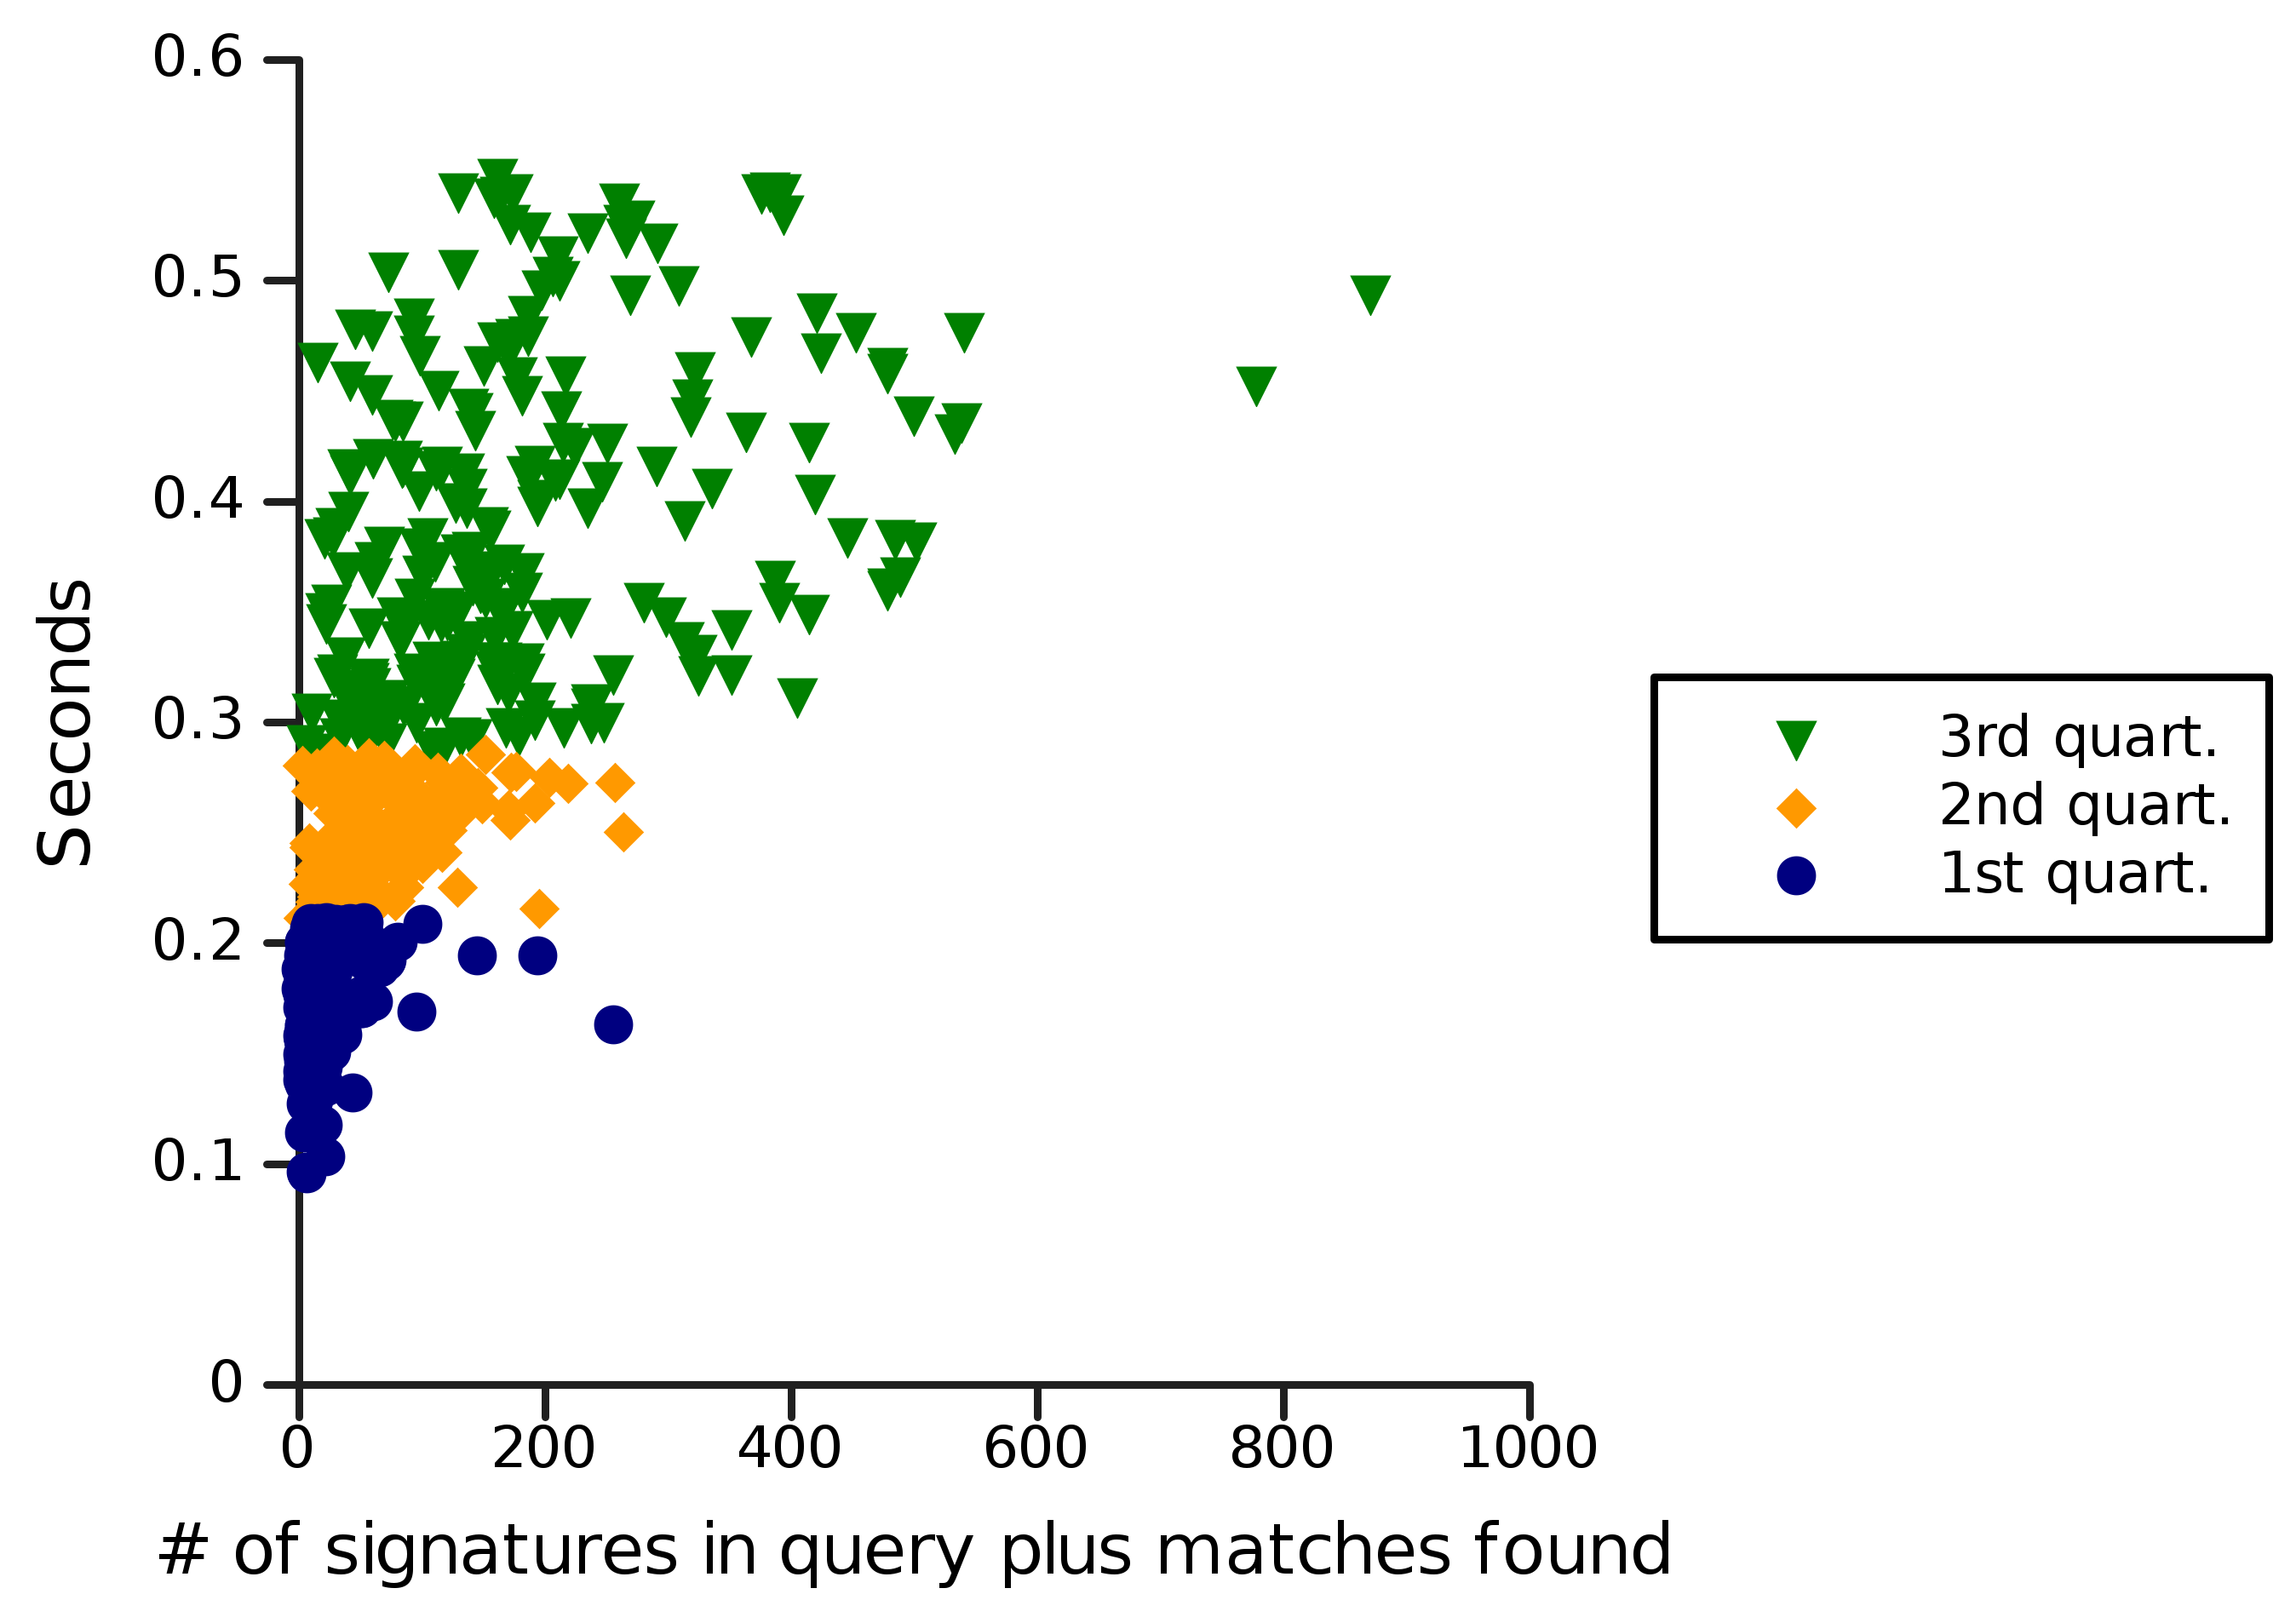
\includegraphics[width=40em]{plots/3quartiles.png}
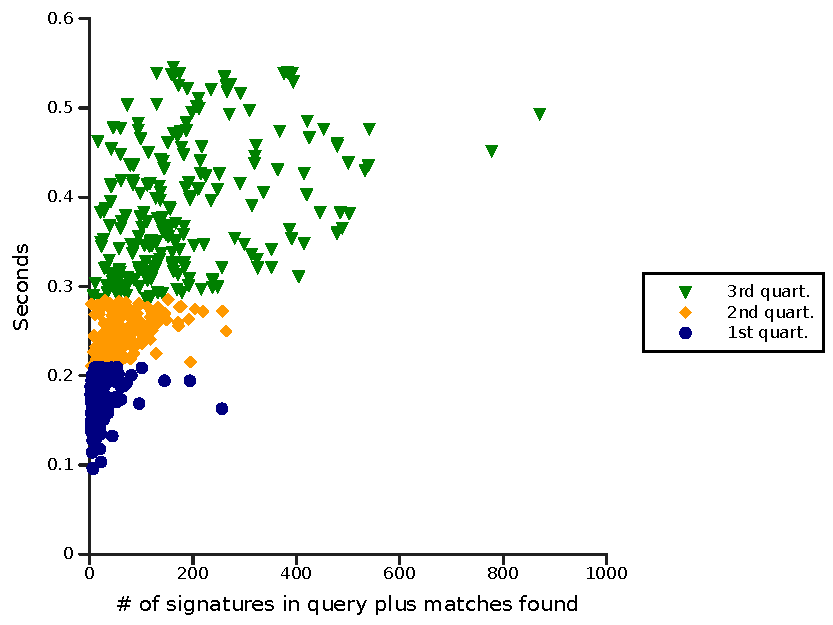
\includegraphics[width=40em]{plots/a.pdf}
  \caption{\small{A closeup on the fastest 75\% of the bin2bin queries (divided
    into quartiles), with q1=fastest, q2=medium fastest, and q3=medium
    slowest.  We plot execution time against a combined tally of results
    returned plus the \# of signatures in the query.  The tally
    models a useful lower-bound on amount of work the database needs to perform.}
}
  \label{fig:perfBin2Bin3quartiles}
\end{figure}
\begin{figure}[h]
  \centering
%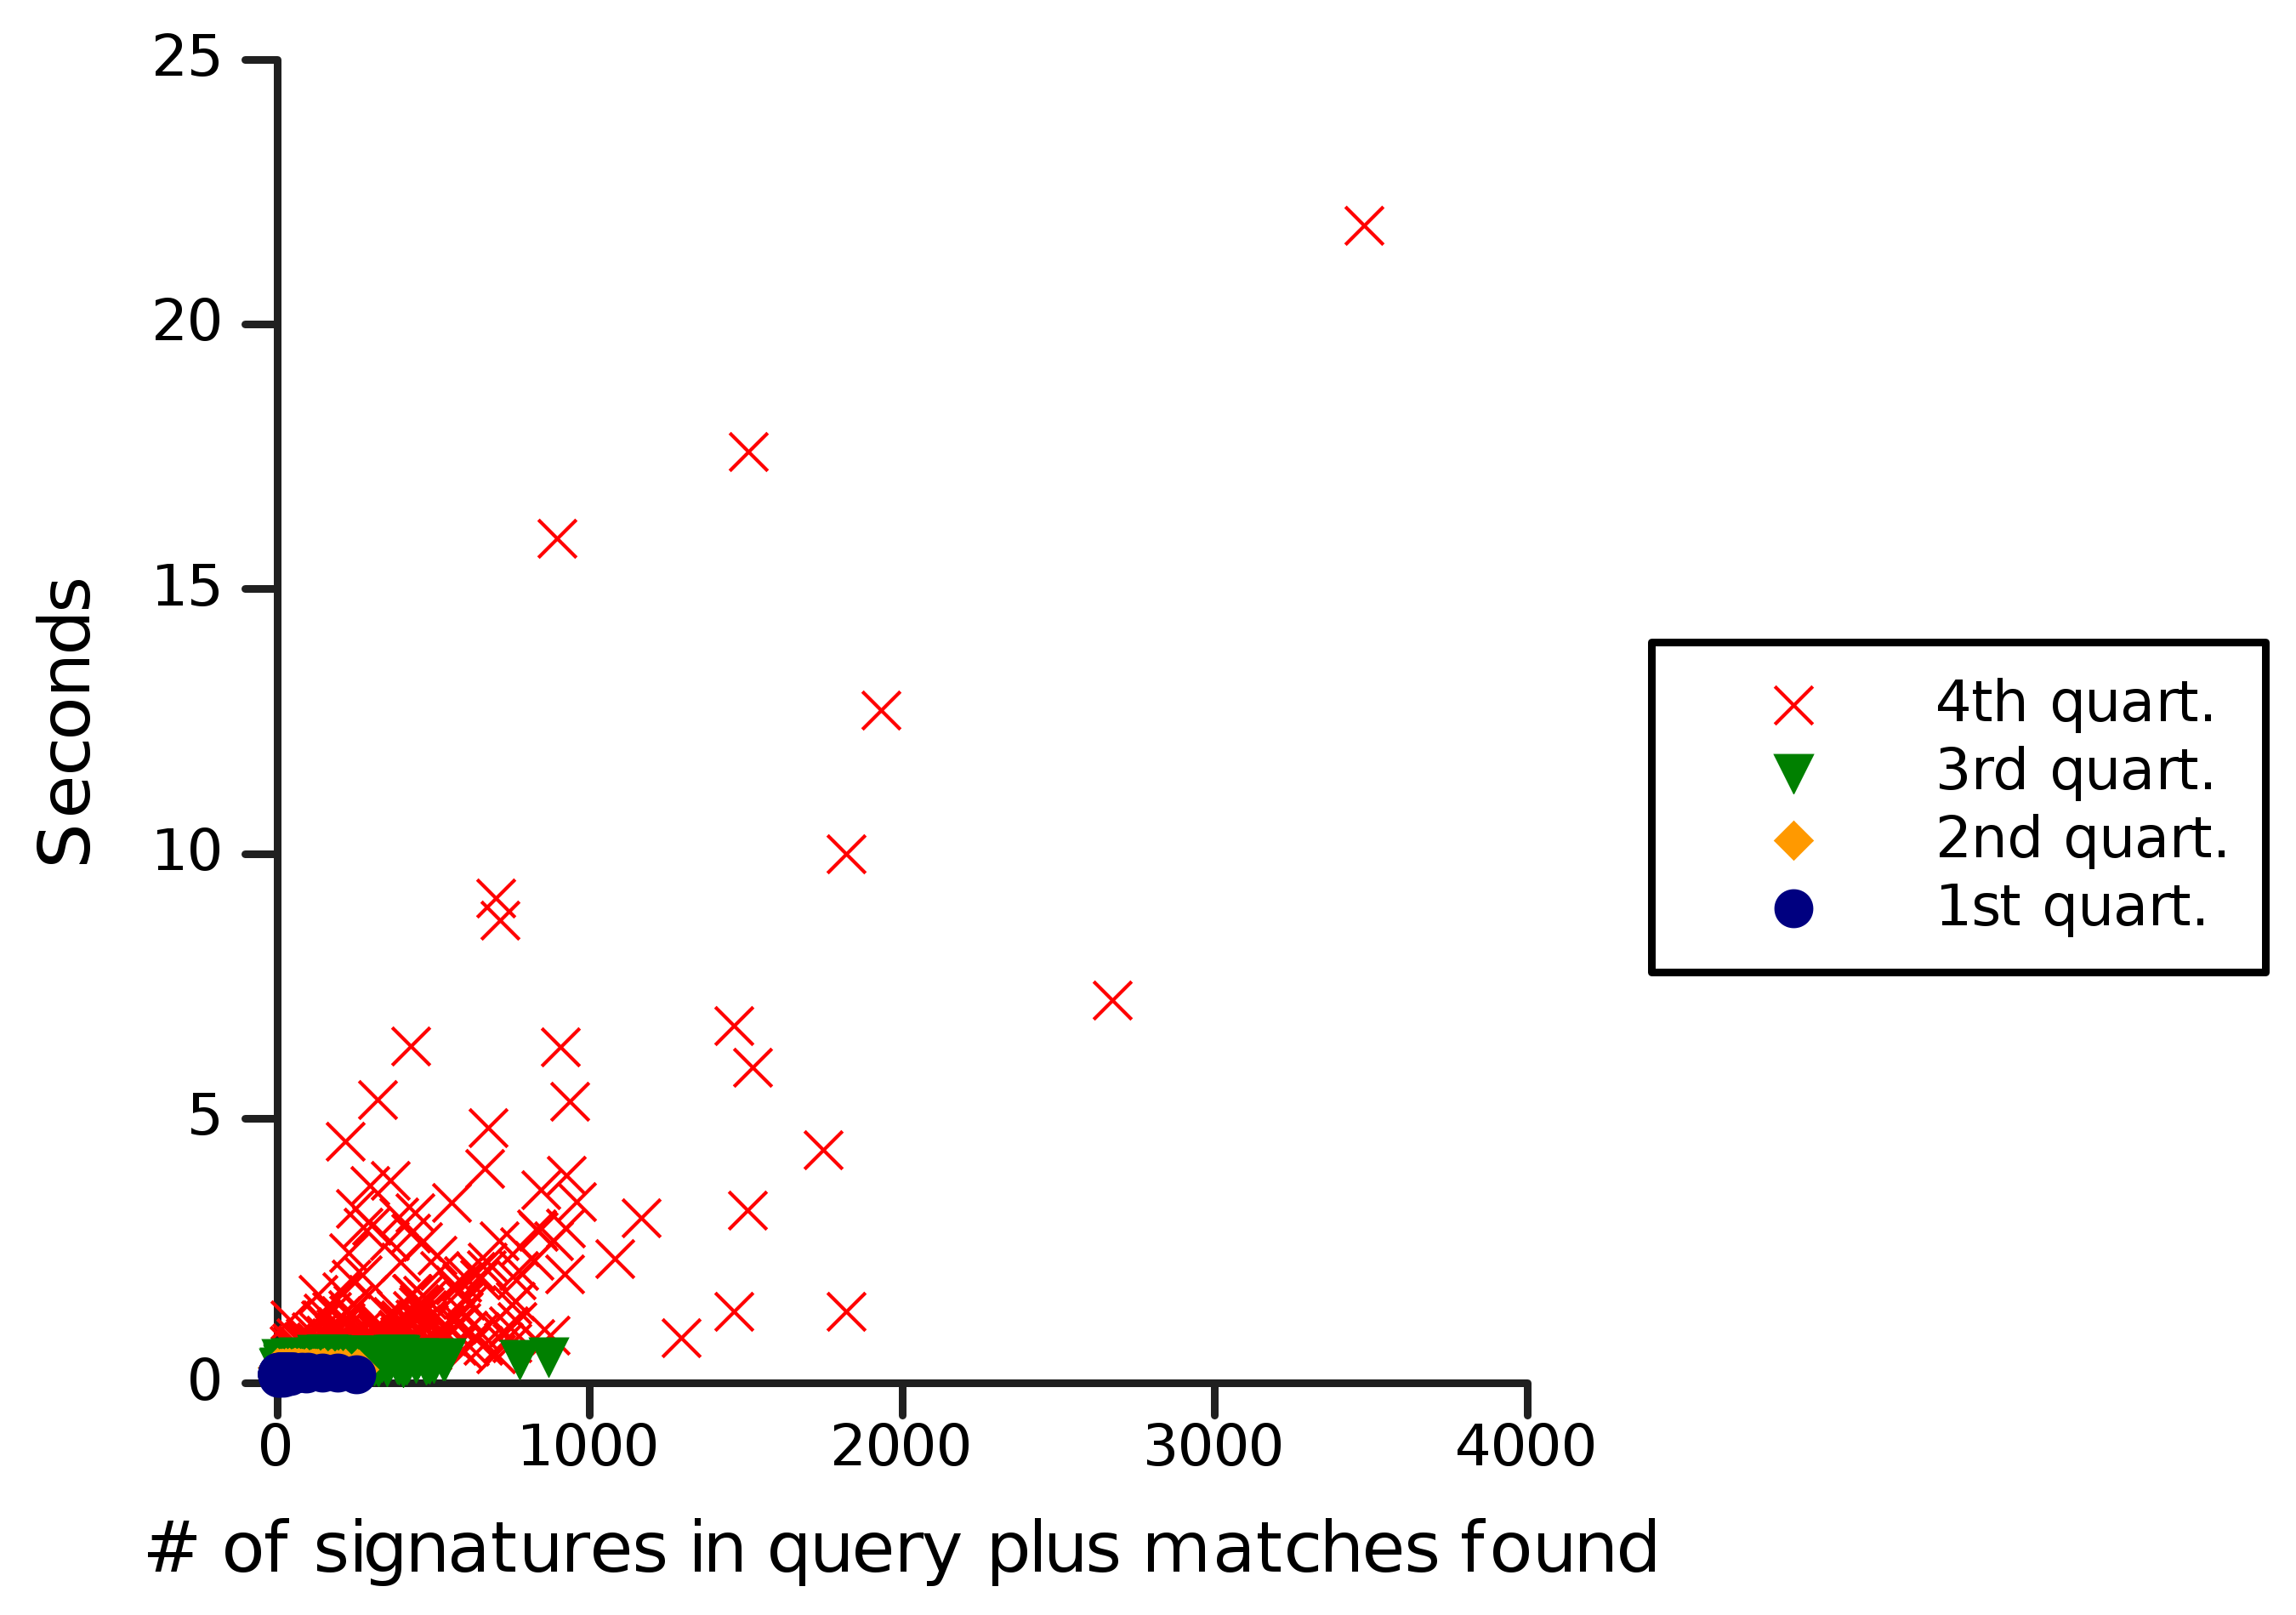
\includegraphics[width=40em]{plots/4quartiles.png}
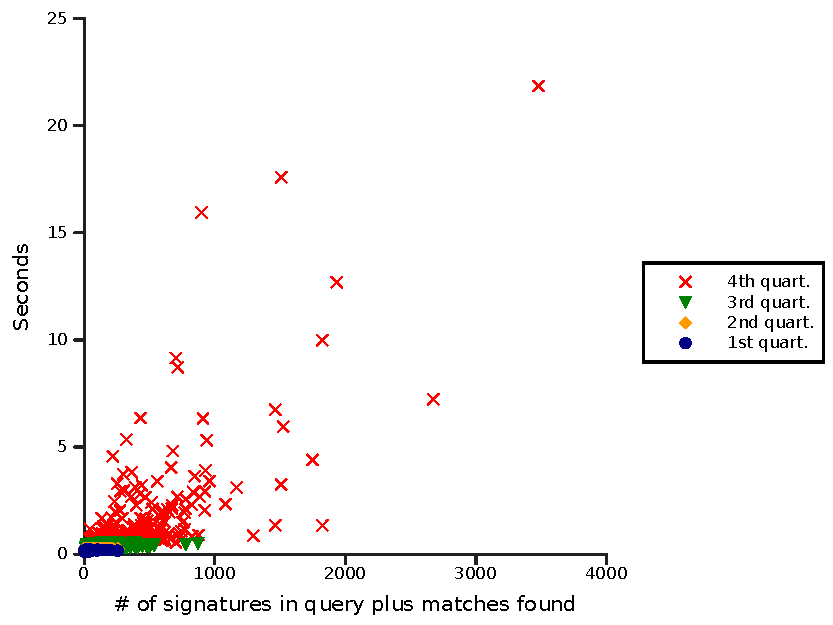
\includegraphics[width=40em]{plots/b.pdf}
\vspace{-2mm}
  \caption{\small{The wide-angle view of the bin2bin query performance (all four
    quartiles), with q1=fastest (barely visible), q2=medium fastest,
    q3=medium slowest, and q4=slowest.  We plot execution time against a
    combined tally of results returned plus the \# of signatures in the
    query.  The tally models a useful lower-bound the amount of work the database needs to
    perform.  The query for \mytt{aspectjtools-1.6.9.jar} in the case study
    took nearly 22 seconds to execute on average.  It contains 2,810
    signatures and its query returns 668 rows.}
}
  \label{fig:perfBin2Bin}
\end{figure}



To summarize, \emph{anchored class signatures} exemplify software Bertillonage:
they are simple, approximate, and significantly faster than exhaustive clone-detection
techniques.   And they are effective.  With most queries requiring on average 2/3rds of a second,
our \emph{anchored class signatures} implementation could be feasibly offered to programmers
within an Integrated Develompent Environment (IDE) such as Eclipse (e.g., right-click on a jar,  click Bertillonage...).
Thanks to previous exhaustive techniques, such as D-CCFinder, it was feasible for programmers,
researchers, and other stakeholders to
run clone-analysis against very large systems.  But they needed a strong case to justify the
time and resource utilization.  With faster light-weight Bertillonage methods, such as
the \emph{anchored class signatures} offered here, provenance analysis
can begin to support stakeholders who \emph{want to know}, as opposed to only those who \emph{need to know}.



%Index queries should perform similar to the Bertillonage techniques, since
%the query structure is identical, but in practice they run faster, due in part
%to the lower frequency of matches (e.g., 2.4 top matches per query compared to
%3.5 for bin2bin).  This makes sense, since any change to a source file,
%even a new comment (and in some cases, a different compiler),
%and certainly any code change, will perturb its
%compiled binary representation, in turn altering its fingerprint, and precluding
%the match.
%This stands in sharp contrast to the Bertillonage class signatures, which are only perturbed by functional
%changes ``outside the curly braces,'' and thus are subject to change by a much smaller set of 
%developer activities.



%\item Debian sample shows that an imperfect corpus can still provide many useful provenance answers.
%      The fact this Debian sample is arguably more challenging from a provenance perspective
%      than what we might expect to observe in nature further strengthens this claim.
%      (e.g., Debian patches sources, uses less common compilers, and has a policy of recompiling).

%\item The industry case study shows how the corpus's own context is important to consider,
%      independent of the corpus's completeness.
%      In this particular example, since the Maven2 repository serves as the main dependency
%      resolver for this particular company, by using the same pool from which the company is obtaining
%      its libraries, we significantly boost the power of the byte-oriented techniques.
%      We also wonder if the company is less likely to consider libraries not already present in Maven2,
%      since such are probably inconvenient for developers to integrate into their existing environments.
                                                                   
%\item Our bin2src experiment sheds some light on how an even further degraded corpus might
%      impact a provenance method.  Source signatures in Maven are 2 times less common, and
%      yet the results in our bin2src experiments were surprisingly decent.






%dmg's bin2src Results:

%\begin{itemize}
%\item 1 same name but .zip instead of .jar (Jaccard 1)
%\item 32 Same name, including -source (max 1.0, min 0.85, median 1.0)
%\item 7 variations of name. Max 1.0, min 0.609, median 0.952. For
%  example: sun-jaxws-2.1.4-20080502-rt and jaxws-rt-2.1.4;19;
%\item 23, variations of version.. We also checked the Inclusion in
%  this one: max 1.0, min 0.113, median 0.929). We checked every one
%  of them and they really looked like different variations in version
%  even those with the lowest Jaccard jdom-1.0.jar and
%  jgom-1.1-sources, with In. 113, and Jaccard .061, the lowest)
%\item 5 False positive (not matched): Min;0.068, Max;0.225,
%  Median;0.200, but even their inclusion is very  low: (Min;0.068,
%  Max;0.225, Median;0.186).
%\item 13 not found. 
%\item For 60, there was only 1 match, for the remainder 21, the min was 2, max, 11, with median of 3. Really narrowing the searching space.
%\item Results changed: now only 20 \emph{1.00} match is a single match, but median for single match is 2
%\end{itemize}





%%% Local Variables: 
%%% mode: latex
%%% TeX-master: "000_main"
%%% End: 
